% Details needed
% Location of Acopian supplies - Nominal current draws
% Location/method of threshold control


\subsection{Drift Chambers}
\label{sec:shmschambers}
The drift chambers provide accurate measurements of particles position
and angles in the detector hut.  This information can be combined with
a knowledge of the spectrometer optics to infer particle momenta and
the angles and positions particles at the target.

\begin{figure}[htb]
\begin{center}
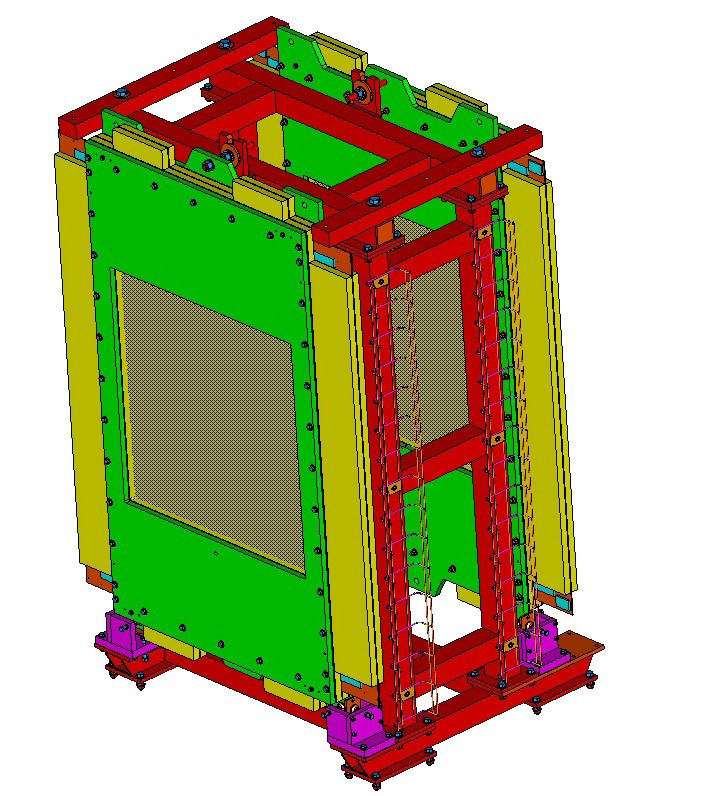
\includegraphics[width=0.75\textwidth]{shms_dcs_frame_drawing.png}
\caption{\label{chamberpair}Technical drawing of the SHMS drift
  chambers mounted in the detector hut frame.}
\end{center}
\end{figure}

The drift chamber package consists of two identical chambers, with 6 planes of
wires each.  (Figure~\ref{chamberpair})  Each wire plane consists of a set of
alternating 20  $\mu\textrm{m}$ gold tungsten sense (anode) wires and 80
$\mu\textrm{m}$ field wires, separated by 0.5cm.  A cathode plane of copper
coated mylar is located between each wire plane, before the first wire plane and
after the last wire plane. In planes labled $X$ and $X^{\prime}$, the wires are
horizontal.  In the $U$ and $U^{\prime}$ planes the wires are rotated
$60^{\circ}$ relative to the $X$ planes while in the $V$ and $V^{\prime}$ planes
the wires are rotated by $-60^{\circ}$.  The
$V^{\prime}$, $X^{\prime}$, and $U^{\prime}$ planes are offset from the unprimed
planes by 0.5 cm.
The first chamber consists of planes
ordered as ($U$, $U^{\prime}$, $X$, $X^{\prime}$, $V^{\prime}$, $V$).  The
second chamber, while of identical design to the first chamber is rotated by
$180^{\circ}$ about the vertical access, so the plane ordering is
($V$, $V^{\prime}$, $X^{\prime}$, $X$, $U^{\prime}$, $U$).  Note however,
this rotation results in the $U$ ($V$) planes in first chamber being parallel
to the $V$ ($U$) planes in the second chamber.
The active area of each chamber is $80~\textrm{cm}\times
80~\textrm{cm}$ which has been set to match the active area for particles in
the SHMS focal plane. Further details about the design and construction of the
drift chambers are in the SHMS Drift Chambers
reference~\cite{howto:shms_drift_chambers}.

The drift chambers 50/50 mixture (by weight) of Ethane/Argon as a
drift gas which
flows across all of the wire planes.  The system that delivers this
gas is described in section~\ref{sec:chambergas}.

The high voltage for the SHMS drift chambers is supplied by CAEN
high voltage, low current, power supplies in the electronics room of
the counting
house and can be controlled through a GUI on the console computers.
The operating voltages for the chambers are a nominal -1800V (foil) and -1800V
(potential wires).  Control of the high voltage system is described in
section~\ref{sec:highvoltage}.

Each anode/sense wire has its own electronic readout through
Nanometrics preamplifier/discriminator cards or LeCroy Corporation LRS
2735DC cards which are interchangeable with the Nanometrics cards.
The discriminator outputs from the cards, each of which instruments 16
sense wires are connected to CAEN V1190 multi-hit TDCs located in the
SHMS electronics hut.
The discriminator cards are powered by +5V and -5V Acopian power
supplies that are
located in the SHMS electronics hut.  The supply currents are several
10s of amps for the positive and negative supplies.
The discriminator thresholds for these cards are controlled by a power
supplies in rack CH03B10 in the Hall C counting house.  Nominal
threshold settings will be posted by on the supply.

\paragraph{Start-of-Run Procedure}
The procedure for turning the chambers on at the start of an
experiment is the following:
\begin{enumerate}
\item Make sure gas is flowing through both chambers.
\item Turn on the low voltage Acopian power supplies in the SOS detector hut.
\item Turn on the FASTBUS power supply if it is not already on.
\item Turn on the threshold power supply to the appropriate setting
  (nominally 1.5V).
\item Turn on the high voltage.
\end{enumerate}

\paragraph{End-of-Run Procedure}
At the end of an experiment or before an extended down, the high
voltage supplies and the Acopian low-voltage supplies should be turned
off.  The ethan gas flow may be shot off, but the argon gas flow
should be left on to keep the chambers clean and dry.

% Add a responsible personell here
